\documentclass[]{article}
\usepackage{lmodern}
\usepackage{amssymb,amsmath}
\usepackage{ifxetex,ifluatex}
\usepackage{fixltx2e} % provides \textsubscript
\ifnum 0\ifxetex 1\fi\ifluatex 1\fi=0 % if pdftex
  \usepackage[T1]{fontenc}
  \usepackage[utf8]{inputenc}
\else % if luatex or xelatex
  \ifxetex
    \usepackage{mathspec}
  \else
    \usepackage{fontspec}
  \fi
  \defaultfontfeatures{Ligatures=TeX,Scale=MatchLowercase}
\fi
% use upquote if available, for straight quotes in verbatim environments
\IfFileExists{upquote.sty}{\usepackage{upquote}}{}
% use microtype if available
\IfFileExists{microtype.sty}{%
\usepackage[]{microtype}
\UseMicrotypeSet[protrusion]{basicmath} % disable protrusion for tt fonts
}{}
\PassOptionsToPackage{hyphens}{url} % url is loaded by hyperref
\usepackage[unicode=true]{hyperref}
\hypersetup{
            pdfborder={0 0 0},
            breaklinks=true}
\urlstyle{same}  % don't use monospace font for urls
\usepackage{longtable,booktabs}
% Fix footnotes in tables (requires footnote package)
\IfFileExists{footnote.sty}{\usepackage{footnote}\makesavenoteenv{long table}}{}
\usepackage{graphicx,grffile}
\makeatletter
\def\maxwidth{\ifdim\Gin@nat@width>\linewidth\linewidth\else\Gin@nat@width\fi}
\def\maxheight{\ifdim\Gin@nat@height>\textheight\textheight\else\Gin@nat@height\fi}
\makeatother
% Scale images if necessary, so that they will not overflow the page
% margins by default, and it is still possible to overwrite the defaults
% using explicit options in \includegraphics[width, height, ...]{}
\setkeys{Gin}{width=\maxwidth,height=\maxheight,keepaspectratio}
\IfFileExists{parskip.sty}{%
\usepackage{parskip}
}{% else
\setlength{\parindent}{0pt}
\setlength{\parskip}{6pt plus 2pt minus 1pt}
}
\setlength{\emergencystretch}{3em}  % prevent overfull lines
\providecommand{\tightlist}{%
  \setlength{\itemsep}{0pt}\setlength{\parskip}{0pt}}
\setcounter{secnumdepth}{0}
% Redefines (sub)paragraphs to behave more like sections
\ifx\paragraph\undefined\else
\let\oldparagraph\paragraph
\renewcommand{\paragraph}[1]{\oldparagraph{#1}\mbox{}}
\fi
\ifx\subparagraph\undefined\else
\let\oldsubparagraph\subparagraph
\renewcommand{\subparagraph}[1]{\oldsubparagraph{#1}\mbox{}}
\fi

% set default figure placement to htbp
\makeatletter
\def\fps@figure{htbp}
\makeatother


\date{}

\begin{document}

\section{Tarea \#6 Red Bayesiana Dinámica (RBD)}\label{header-n0}

\begin{itemize}
\item
  Luis Ernesto Ibarra Vázquez C511s
\item
  Luis Enrique Dalmau Coopat C511
\end{itemize}

\subsection{Descripción Teórica de RBD}\label{header-n7}

\subsubsection{Representación}\label{header-n8}

Las RBD son una extensión de las RB para modelar ditribuciones de
probabiliad de secuencias sobre una colección semi-infinitas de
variables aleatorias. El término dinámico se refiere a que se modela un
sistema dinámico, no que la red cambia con el tiempo, aunque existen
modelos que pueden hacerlo. Para la representación del instante de
tiempo, las variables se sufijan con el número correspondiente a este.

Una RBD esta compuesta por un par ($B1$, $B_{arrow}$) en
donde B1 define la distribución del estado inicial en el tiempo y
$B_arrow$ es una two-slice Temporal Bayes Network (2TBN) que define la
transición entre el estado $Z_{t-1}$ al $Z_t$, o sea
$P(Z_t|Z_{t-1})$, esta es representada por un grafo
dirigido acíclico. La definición anterior trae implícita la propiedad
Markoviana de las RBD entre diferentes tiempos, $(Z_{t+1} \perp Z_{t-1} | Z_{t})$.

$$P(Z_t|Z_{t-1}) = \Pi_{i=1}^{N} P(Z_t^i|Pa(Z^i_t))$$

Donde $Z_t^i$ es el i-ésimo nodo en tiempo t.

\begin{figure}
\centering
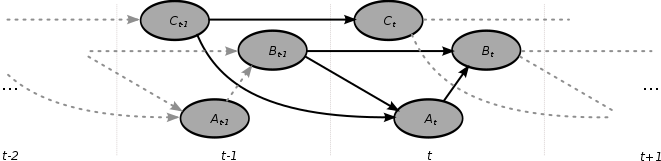
\includegraphics{images/2TSBN.png}
\caption{}
\end{figure}

En la figura anterior se representa una posible definición de una
$B_{arrow}$ de una RBD.

Generalmente las variables $Z_t$ se dividen en tres grupos,
variables ocultas $X_t$, variables observables $Y_t$ y variables de
control $U_t$. Las variables ocultas son estados no observados en el
proceso modelado, las variables observables son estados observados del
proceso y las variables de control son estados impuestos por medios
externos al modelo que pueden influenciar las variables ocultas de este.

Los Modelos Ocultos de Markov (MOM) y los Modelos Filtros de Kalman
(MFK) son casos específicos de estas, demostrando así su gran poder
expresivo de las RBD.

\textbf{Modelo Oculto de Markov como RBD}

\begin{figure}
\centering
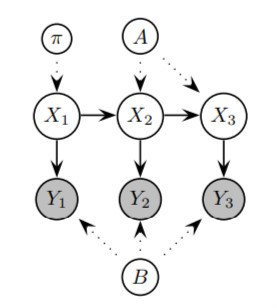
\includegraphics{images/HMMasDBN.jpg}
\caption{}
\end{figure}

Donde:

\begin{itemize}
\item
  $\pi$: Distribución inicial de $X_1$
\item
  $X_i$: Variable Oculta en el time-slice i
\item
  $Y_i$: Variable Observada en el time-slice i
\item
  $A$: Matriz estocástica de transición entre Estados Ocultos
\item
  $B$: Matriz estocástica de observación entre el Estado Oculto y el
  Estado Observado (Caso Discreto)
\end{itemize}

\textbf{Modelo Filtro de Kalman como RBD}

La representación es similar al MOM, ya que ambos asumen lo mismo, la
diferencia radica en que las variables de MFK son variables continuas
que distribuyen normal.

\subsubsection{Inferencia}\label{header-n33}

\textbf{Algoritmo forwards-backwards}

Para el caso discreto de una RBD se convierte esta en un Modelo Oculto
de Markov y se aplica sobre esta nueva red el algoritmo antes
mencionado:

Se define:

$$\alpha_t(i) = P(X_t = i | y_{1:t})$$

$$\beta_t(i) = P(y_{t+1:T} | X_t=i)$$

$$\gamma_t(i) = P(X_t=i | y_{1:T}) = \frac{1}{P(y_{1:T})} \alpha_t(i) * \beta_t(i)$$

Este algoritmo tiene dos pasos, el paso hacia adelante en el que se
calcula $\alpha_t$ y el paso hacia atrás en donde
se calcula $\beta_t$ para conocer el objetivo del
cálculo $\gamma_t$.

En el paso hacia adelante se computa recursivamente $\alpha_t$

$$\alpha_t(j) = P(X_t = j|y_{1:t}) = \frac{1}{c_t}P(X_t = j, y_t|y_{1:t-1})$$

Donde

$$P(X_t = j, y_t|y_{1:t-1}) = (\sum_i P(X_t = j | X_{t-1} = i) P(X_{t-1}=i|y_{1:t-1})) P(y_t|X_t=j)$$

y

$$c_t = P(y_t|y_{1:t-1}) = \sum_j P(X_t = j, y_t | y_{1:t-1})$$

En la definición de la RBD se tienen las distribuciones de:

$$P(X_t = j | X_{t-1} = i) \quad y \quad P(y_t|X_t=j)$$

Que son las probabilidades de transición y emisión respectivamente del
modelo de Markov. Por lo que la expresión que queda es:

$$\alpha_{t-1}(i) = P(X_{t-1}=i|y_{1:t-1})$$

En el paso hacia atrás:

Se tiene como caso base

$$\beta_T(i) = 1 = Pr(y_{T+1:T}|X_T=i) = Pr(\emptyset|X_T = i)$$

El paso recursivo es:

$$P(y_{t+1:T}| X_t = i) = \sum_j P(y_{t+2:T}, X_{t+1}=j, y_{t+1})$$

$$P(y_{t+1:T}| X_t = i) = \sum_j P(y_{t+2:T}| X_{t+1}=j, y_{t+1}, X_t=i) P(X_{t+1}=j, y_{t+1}|X_t = i)$$

$$P(y_{t+1:T}| X_t = i) = \sum_j P(y_{t+2:T}| X_{t+1}=j) P(y_{t+1}| X_{t+1}=j)P(X_{t+1}=j, y_{t+1}|X_t = i)$$

$$\beta_{t}(i) = \sum_j \beta_{t+1}(j) P(y_{t+1}| X_{t+1}=j)P(X_{t+1}=j, y_{t+1}|X_t = i)$$

Donde igualmente se las expresiones restantes en la definición de la
RBD.

Finalmente con las expresiones de $\alpha$ y
$\beta$ se calcula $\gamma$.

\subsection{Descripción Práctica}\label{header-n61}

Las RBD están presentes en el Procesamiento del Lenguaje Natural (PLN).
En este campo son usadas en la anotación de etiquetas de partes de la
oración o Part of Speech (POS) en inglés. Existen varios conjuntos de
etiquetas POS, en este trabajo nos centraremos en etiquetas consideradas
universales por los corpus usados:

\begin{longtable}[]{@{}lll@{}}
\toprule
Tag & Meaning & English Examples\tabularnewline
\midrule
\endhead
ADJ & adjective & new, good, high, special, big, local\tabularnewline
ADP & adposition & on, of, at, with, by, into, under\tabularnewline
ADV & adverb & really, already, still, early, now\tabularnewline
CONJ & conjunction & and, or, but, if, while, although\tabularnewline
DET & determiner & , article the, a, some, most, every, no,
which\tabularnewline
NOUN & noun & year, home, costs, time, Africa\tabularnewline
NUM & numeral & twenty-four, fourth, 1991, 14:24\tabularnewline
PRT & particle & at, on, out, over per, that, up, with\tabularnewline
PRON & pronoun & he, their, her, its, my, I, us\tabularnewline
VERB & verb & is, say, told, given, playing, would\tabularnewline
. & punctuation & marks . , ; !\tabularnewline
X & other & ersatz, esprit, dunno, gr8, univeristy\tabularnewline
\bottomrule
\end{longtable}

El problema anterior consiste en dado una secuencia de tokens, devolver
cada token anotado con su etiqueta POS correspondiente. Por ejemplo:

\begin{longtable}[]{@{}llllll@{}}
\toprule
El & perro & peludo & ladra & y & juega\tabularnewline
\midrule
\endhead
DET & NOUN & ADJ & VERB & CONJ & VERB\tabularnewline
\bottomrule
\end{longtable}

Este tipo de anotación es usado como atributos en múltiples tareas de
PLN por lo que tiene una gran importancia teórica y práctica.

\subsubsection{Modelación}\label{header-n133}

Se creó un algoritmo que generaliza el anotado de POS para una
estructura particular de RBD. En la RBD propuesta las variables se
dividen en dos secciones, las variables observadas y las variables
ocultas. Las variables observadas corresponden a características de la
palabra observada de la secuencia, como por ejemplo su longitud, si
empieza con mayúsculas. Las variables ocultas corresponden a
características no observadas de la palabra como es el caso de la
etiqueta POS de ella. El tiempo se modeló como la posición de la palabra
en una oración.

El modelado corresponde al siguiente grafo:

\begin{figure}
\centering
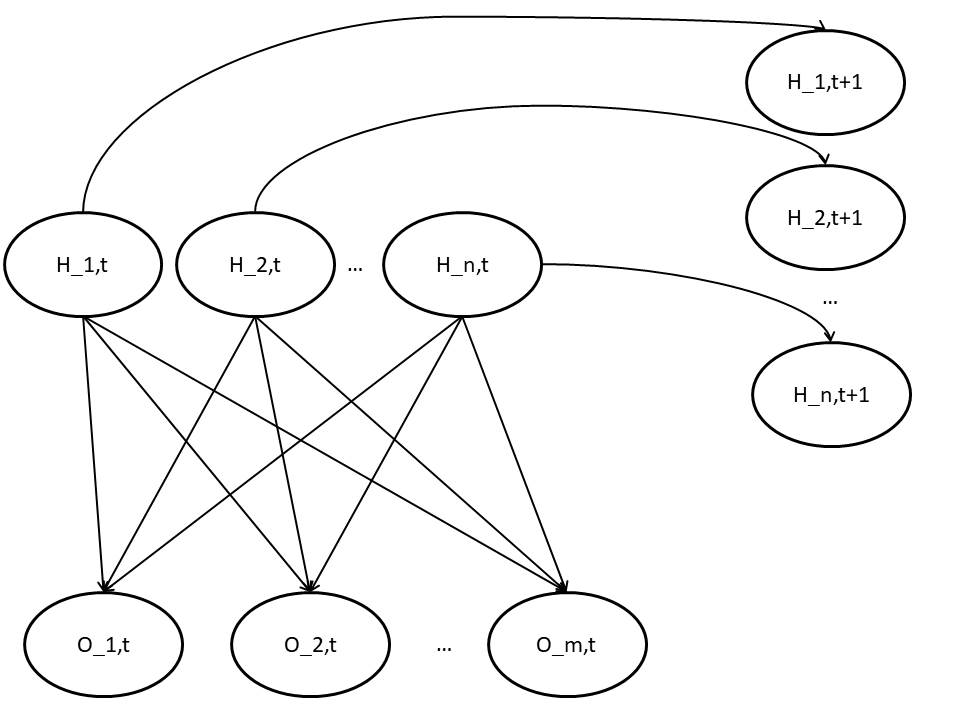
\includegraphics{F:/Universidad/Quinto/1er_Semestre/CO Modelos Gráficos Probabilistas/Tareas/grupo_Ibarra-Dalmau/images/DBN.jpg}
\caption{}
\end{figure}

En el modelo se observa la definición de una 2TBN. En el caso particular
del problema a resolver existe solo una variable oculta, la etiqueta
POS, pero se puede extender a que múltiples variables ocultas con
facilidad. La restricción de las variables ocultas ($H_i$,$t$)
es que solo se conectan con su correspondiente en el intervalo de tiempo
siguiente ($H_i$,$t+1$) y que se conectan con todas las variables
observadas en su intervalo de tiempo ($O_i$,$t$). Lo interesante de
este modelo es la flexibilidad con que se pueden añadir atributos
observables.

El modelo concreto implementado se observa en la siguiente figura,
añadiendo la posibilidad de agregar nuevos atributos:

\begin{figure}
\centering
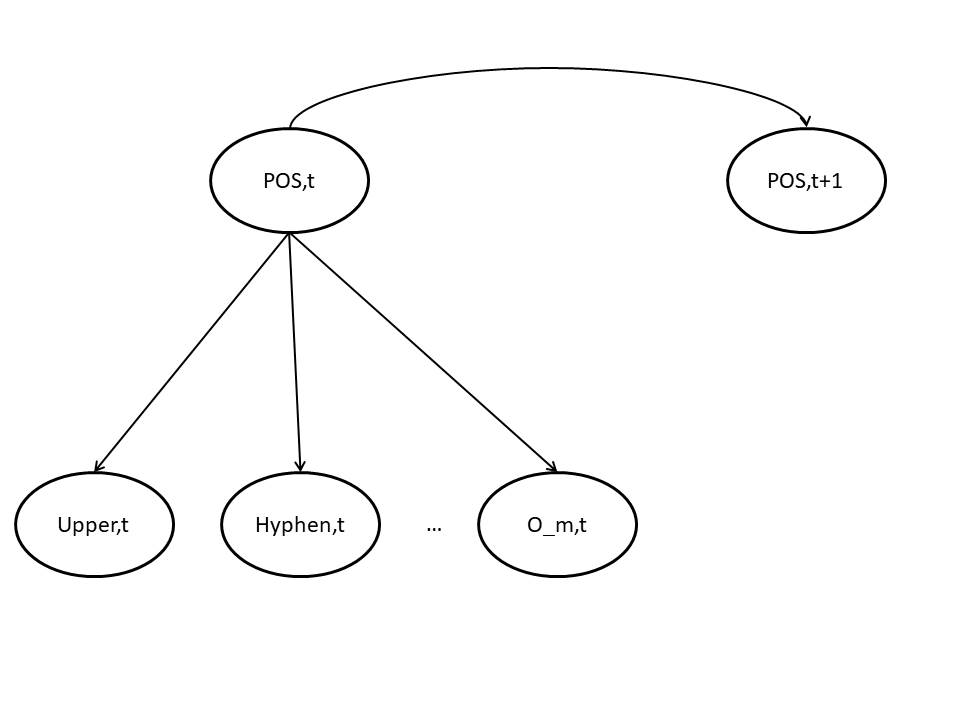
\includegraphics{images/DBN_POS.jpg}
\caption{}
\end{figure}

\subsubsection{Entrenamiento}\label{header-n140}

Para el entrenamiento se construyeron las tablas de la red usando los
bigramas encontrados en el corpus para aprender las distribuciones de
las variables.

Se particionó el corpus en 2 conjuntos, el conjunto de entrenamiento y
el conjunto de pruebas, con una proporción de 70\%-30\% respectivamente.

\subsubsection{Algoritmo}\label{header-n143}

El algoritmo se basa en tomar la etiqueta POS más probable de la palabra
dados la etiqueta POS anterior y los valores de las variables observadas
de la palabra en cuestión. Este proceso se repite hasta que se acaben la
palabra teniendo al final la cadena anotada con las etiquetas POS
correspondientes.

$$POS_t = arg \max_i P(POS_t = i | POS_{t-1}, Obs_t)$$

\subsubsection{Software}\label{header-n146}

Para la implementación del modelo nos basamos en la biblioteca
\textbf{pgmpy}. En este usamos las definiciones de Red Bayesiana y de
Red Dinámica Bayesianas ya implementadas, además de los algoritmos de
inferencia que actúan sobre ellas. Para la obtención del corpus nos
basamos en \textbf{nltk}, en esta biblioteca existen múltiples conjuntos
de datos con oraciones que tienen las etiquetas POS anotadas.
Particularmente nos concentramos en el corpus Brown, el cual es una
colección de muestras de textos en inglés americano estructurado en
varios géneros.

\subsubsection{Resultados}\label{header-n148}

El conjunto de variables observadas elegido fue un sencillo conjunto de
dos variables, estas son si la letra comienza con mayúscula y si la
palabra contiene un - en ella. Se entrenó el modelo con el corpus de
Brown de nltk. El resultado fue una precisión del 40\%. Aunque resultado
es bajo con respecto al estado del arte del problema que se encuentra
por encima del 95\%, es superior a un anotador random, el cual con el
conjunto universal de etiquetas alcanzaría aproximadamente un 8\%
(1/|Cantidad de etiquetas POS|).

Luego se realizó una mejora al modelo agregándole más información sobre
las palabras por medio de añadirle más variables observadas. Las
agregadas fueron las variables si la palabra es un número y si la
palabra contiene un signo de puntuación. Con esta modificación se logró
alcanzar un 50\% de precisión en las pruebas.

\begin{longtable}[]{@{}llll@{}}
\toprule
& Baseline & RBD (Upper, Hyphen) & RBD (Upper, Hyphen, Num,
Punct)\tabularnewline
\midrule
\endhead
Precisión & 8\% & 40\% & 50\%\tabularnewline
\bottomrule
\end{longtable}

Los resultados anteriores puede ser posible mejorarlos con la
investigación de un conjunto de atributos que puedan ayudar a mejorar la
identificación de las variables ocultas. Esto se pudo observar en la
modificación al agregarle las variables en el segundo experimento.

\subsection{Referencias}\label{header-n163}

\begin{itemize}
\item
  Dynamic Bayesian Networks: Representation, Inference and Learning
  (Suresh Babu)
\item
  https://www.nltk.org/book/ch05.html
\item
  Probabilistic Graphical Models Principles and Techniques MIT 2009
\item
  https://pgmpy.org/exact\emph{infer/dbn}infer.html
\item
  https://pgmpy.org/param\_estimator/mle.html
\item
  https://pgmpy.org/param\emph{estimator/bayesian}est.html
\item
  https://en.wikipedia.org/wiki/Brown\_Corpus
\end{itemize}

\end{document}
